\subsection{Gran Breta~na}
En esta instancia de experimentaci'on vamos a analizar las rutas a la universidad de Oxford, ubicada en Inglaterra, utilizando la direcci'on \textit{ox.ac.uk}. 
El origen del mensaje es una direcci'on en Argentina y en un principio esperamos, basados en los mapas de cables submarinos, ver 2 o m'as saltos intercontinentales. Si bien
existen caminos con 2 saltos intercontinentales, podria ser 3 si una ruta pasa por europa continental. 

Utilizando 30 repeticiones por cada TTL conseguimos los siguientes datos


\begin{tabular}{ |p{2cm}||p{3cm}|p{3cm}|p{3cm}|  }
 \hline
 \multicolumn{4}{|c|}{Traceroute a Oxford} \\
 \hline
 \textit{TTL} & \textit{IP}  & \textit{RTT} & $\delta$\textit{RTT} \\
 \hline
 0   & 192.168.1.1   & 2.18 ms &   -\\
 1   & Sin respuesta  & - &   -\\
 2   & Sin respuesta  & - &   -\\
 3   & Sin respuesta  & - &   -\\
 4   & Sin respuesta   & - &   -\\
 5   & 200.89.161.97  & 31.49 ms &  29.3 ms\\
 6   & 200.89.165.197  & 29.2 ms &  - \\
 7   & 200.89.165.222  & 34.88 ms &  3.4 ms\\
 8   & Sin respuesta  & - &   -\\
 9   & 67.17.94.249 x & 24.74 ms &  22.7 ms\\
 10   & Sin respuesta   & - &   -\\
 11   & Sin respuesta   & - &   -\\
 12   & 212.187.139.166  & 24.74 ms &  22.7 ms\\
 13   & 146.97.35.197   & 24.74 ms &  22.7 ms\\
 14   & 1146.97.33.2  & 24.74 ms &  22.7 ms\\
 15   & 146.97.37.194   & 24.74 ms &  22.7 ms\\
 16   & 193.63.108.94   & 24.74 ms &  22.7 ms\\
 17   & 193.63.108.98   & 24.74 ms &  22.7 ms\\
 18   & 193.63.109.90   & 24.74 ms &  22.7 ms\\
 19   & Sin respuesta   & - &   -\\
 20   & 192.76.32.62   & 24.74 ms &  22.7 ms\\
 21   & 129.67.242.154   & 24.74 ms &  22.7 ms\\
 \hline
\end{tabular}


Los paquetes con \textit{TTL} 1 a 4 pertenecientes al proveedor de internet no responden 
(sabemos esto ya que los siguientes tambi'en pertenecen al proveedor) creemos que es porque son dispositivos que priorizan otras tareas y deciden no
responder con un mensaje utilizando sus recursos m'as eficientemente.

TODO Mencionar outliers, saltos pelotudos que son menores que sus antecesores, saltos intercontinentales, clusters.


\begin{figure}[!h]
\centering
\caption{TODO}
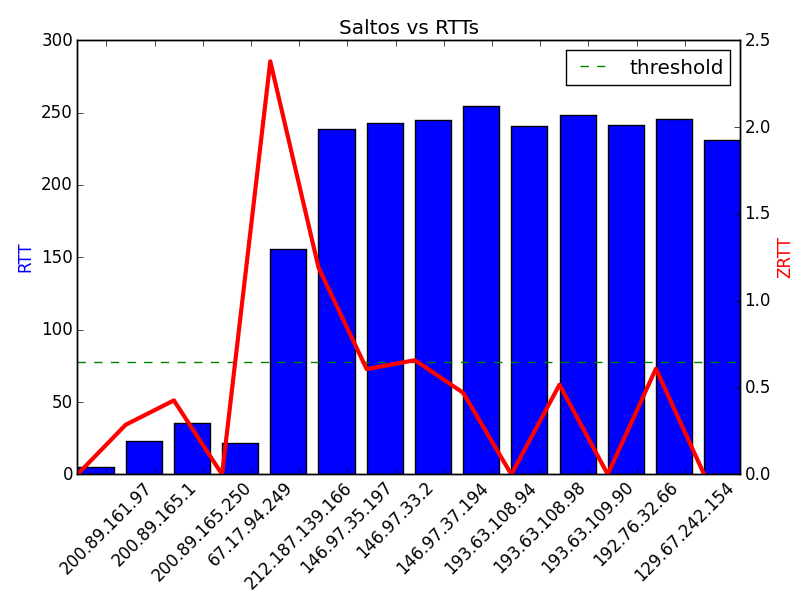
\includegraphics[width=0.75\textwidth]{modules/oxford_rtts}
 \label{fig:oxford_rtts}
\end{figure}


\begin{figure}[!h]
\centering
\caption{TODO}
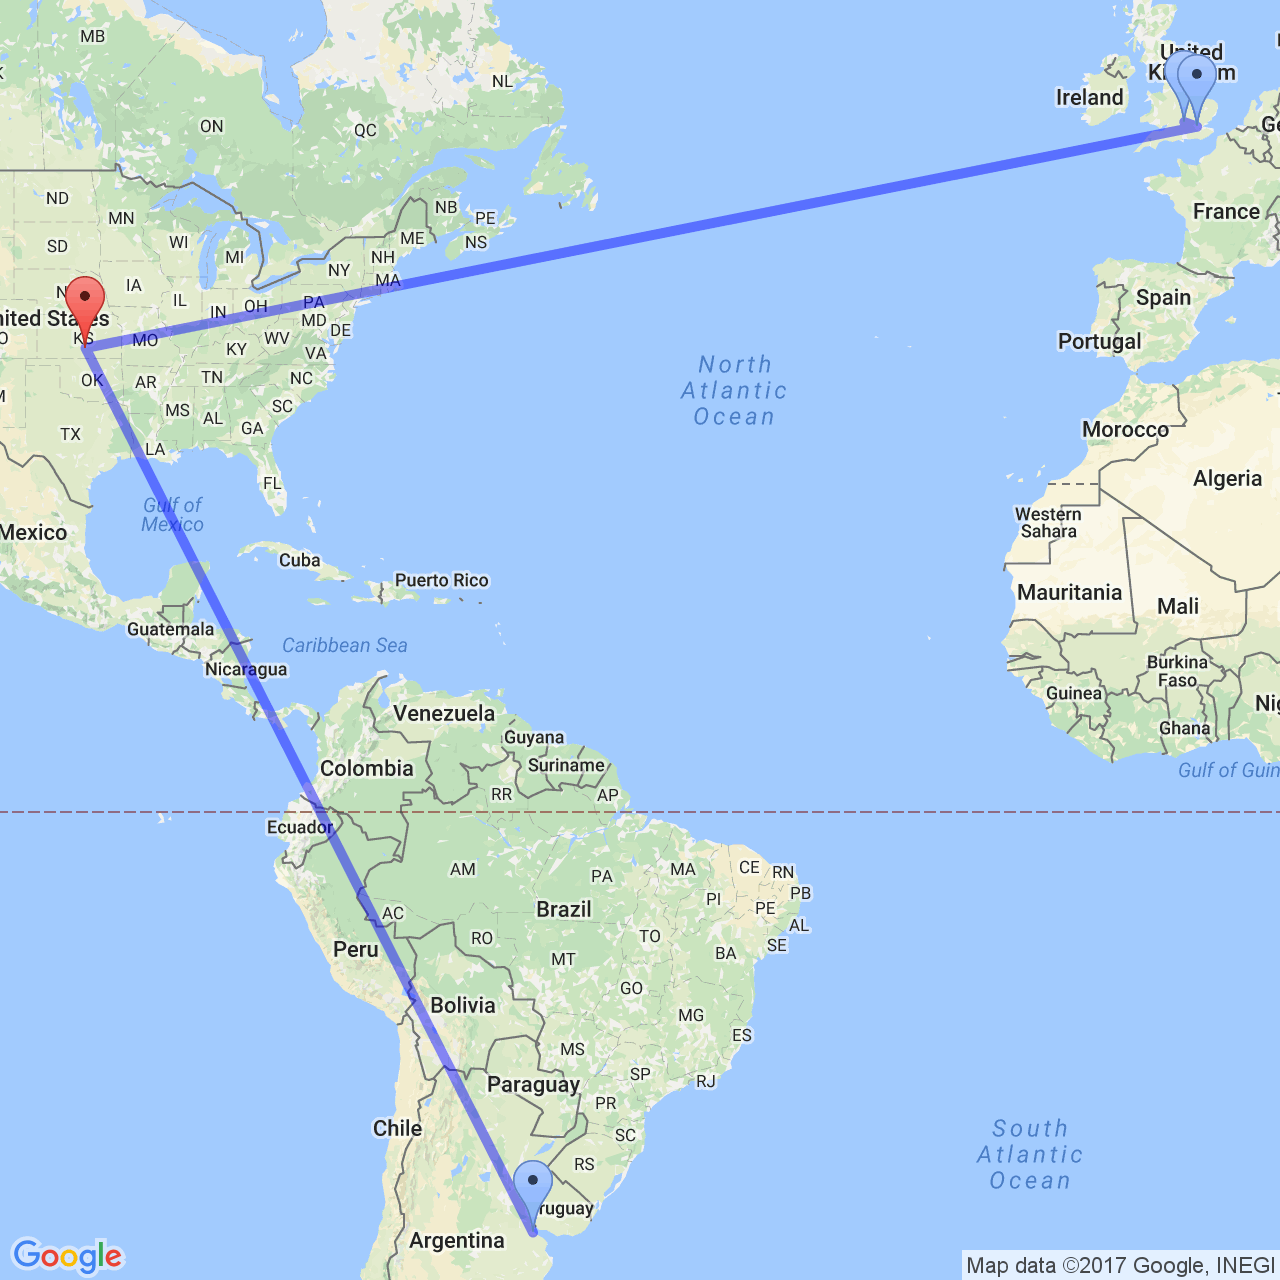
\includegraphics[width=0.75\textwidth]{modules/oxford_path_1}
 \label{fig:ruta_oxford_1}
\end{figure}


\begin{figure}[!h]
\centering
\caption{TODO}
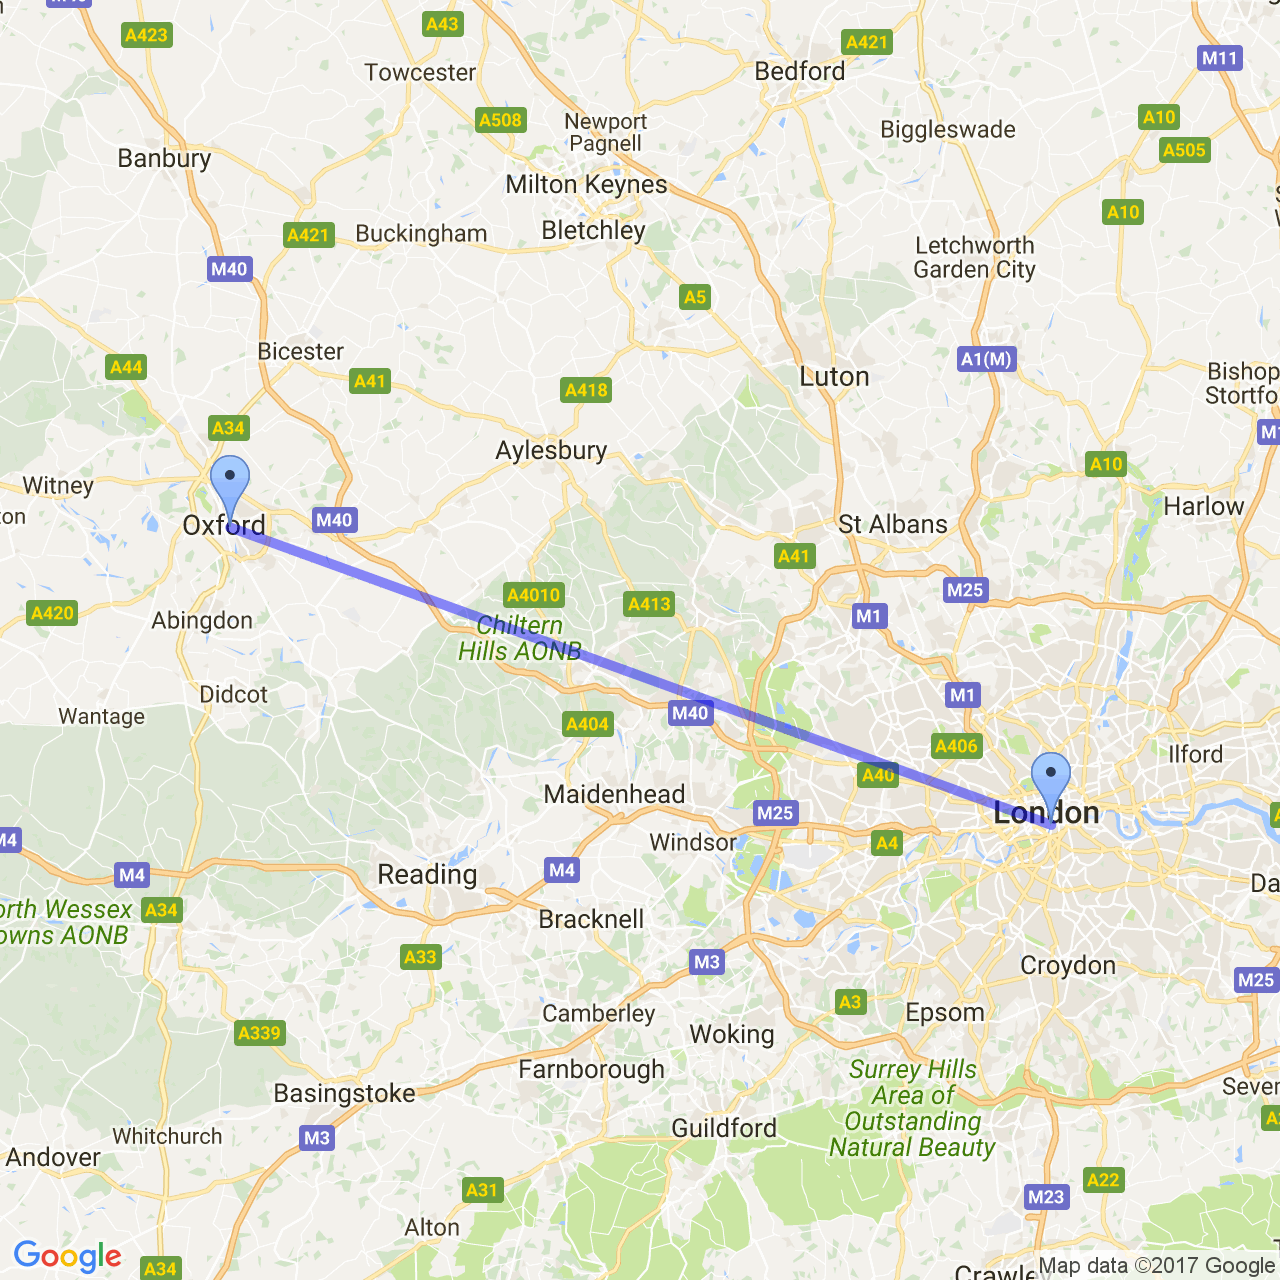
\includegraphics[width=0.75\textwidth]{modules/oxford_path_2}
 \label{fig:ruta_oxford_2}
\end{figure}
